% 1) Title
% 2) Date
% 3) Location
% 4) Present
% 5) Picture
% 6) Start Time
% 7) Stop Time
\insertmeeting 
	{Helping Heroes} 
	{09/01/21}
	{Hagerty High School}
	{Jensen, Nathan, Ritam}
	{Images/RobotPics/robot.jpg}
	{1:30}
 	{3:30}
	
\section*{Outreach}
\noindent\hfil\rule{\textwidth}{.4pt}\hfil
\subsection*{Goals}
\begin{itemize}
    \item Teach 4227 members CAD basics
    \item Get to know 4227 members better

\end{itemize} 

\noindent\hfil\rule{\textwidth}{.4pt}\hfil

\subsection*{Accomplishments}
Today was our sister team, 4227 Metal Morphosis' first full robotics meeting. This would be the first time they would start working on robotics related things, and today they started with CAD. A few meetings ago they created onshape accounts, but they hadn’t begun learning it yet. In order to help them learn, several members of our hardware committee went to help them learn. We started out by giving a quick rundown of what CAD is and the basics of how it works. We then broke off and worked one on one with 4227 members, taking turns so everyone had an opportunity to learn.  Everyone got to try to make the first letter of their name, with some help from us 4717 members (image 1&2). This allowed them to learn how to make sketches, extrudes, chamfer, and fillets, all tools that we use regularly when designing our robots. For some of the 4227 members that were more interested in working with CAD in the future, we went into a bit more depth, showing them how to create assemblies and insert standard content, like screws and nuts (image 3). Overall they were able to make good progress in learning CAD and should be better prepared for the upcoming season.

\begin{figure}[ht]
\centering
\begin{minipage}[b]{.50\textwidth}
  \centering
  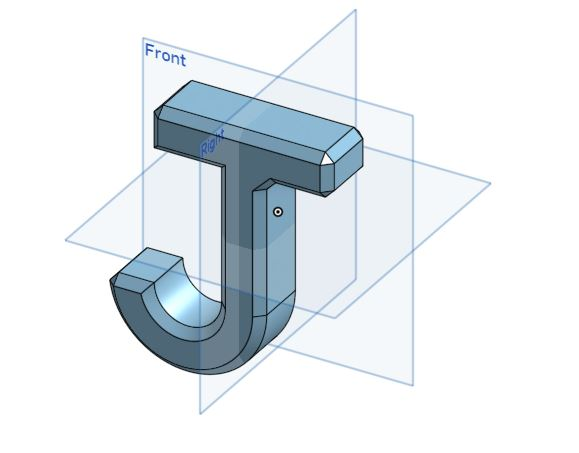
\includegraphics[width=0.8\textwidth]{Meetings/September/09-01-21/9-1-21_Program_Image1 - Nathan Forrer.JPG}
  \caption{Jorge's First Name}
  \label{fig:pic1}
\end{minipage}%
\hfill%
\begin{minipage}[b]{.50\textwidth}
  \centering
  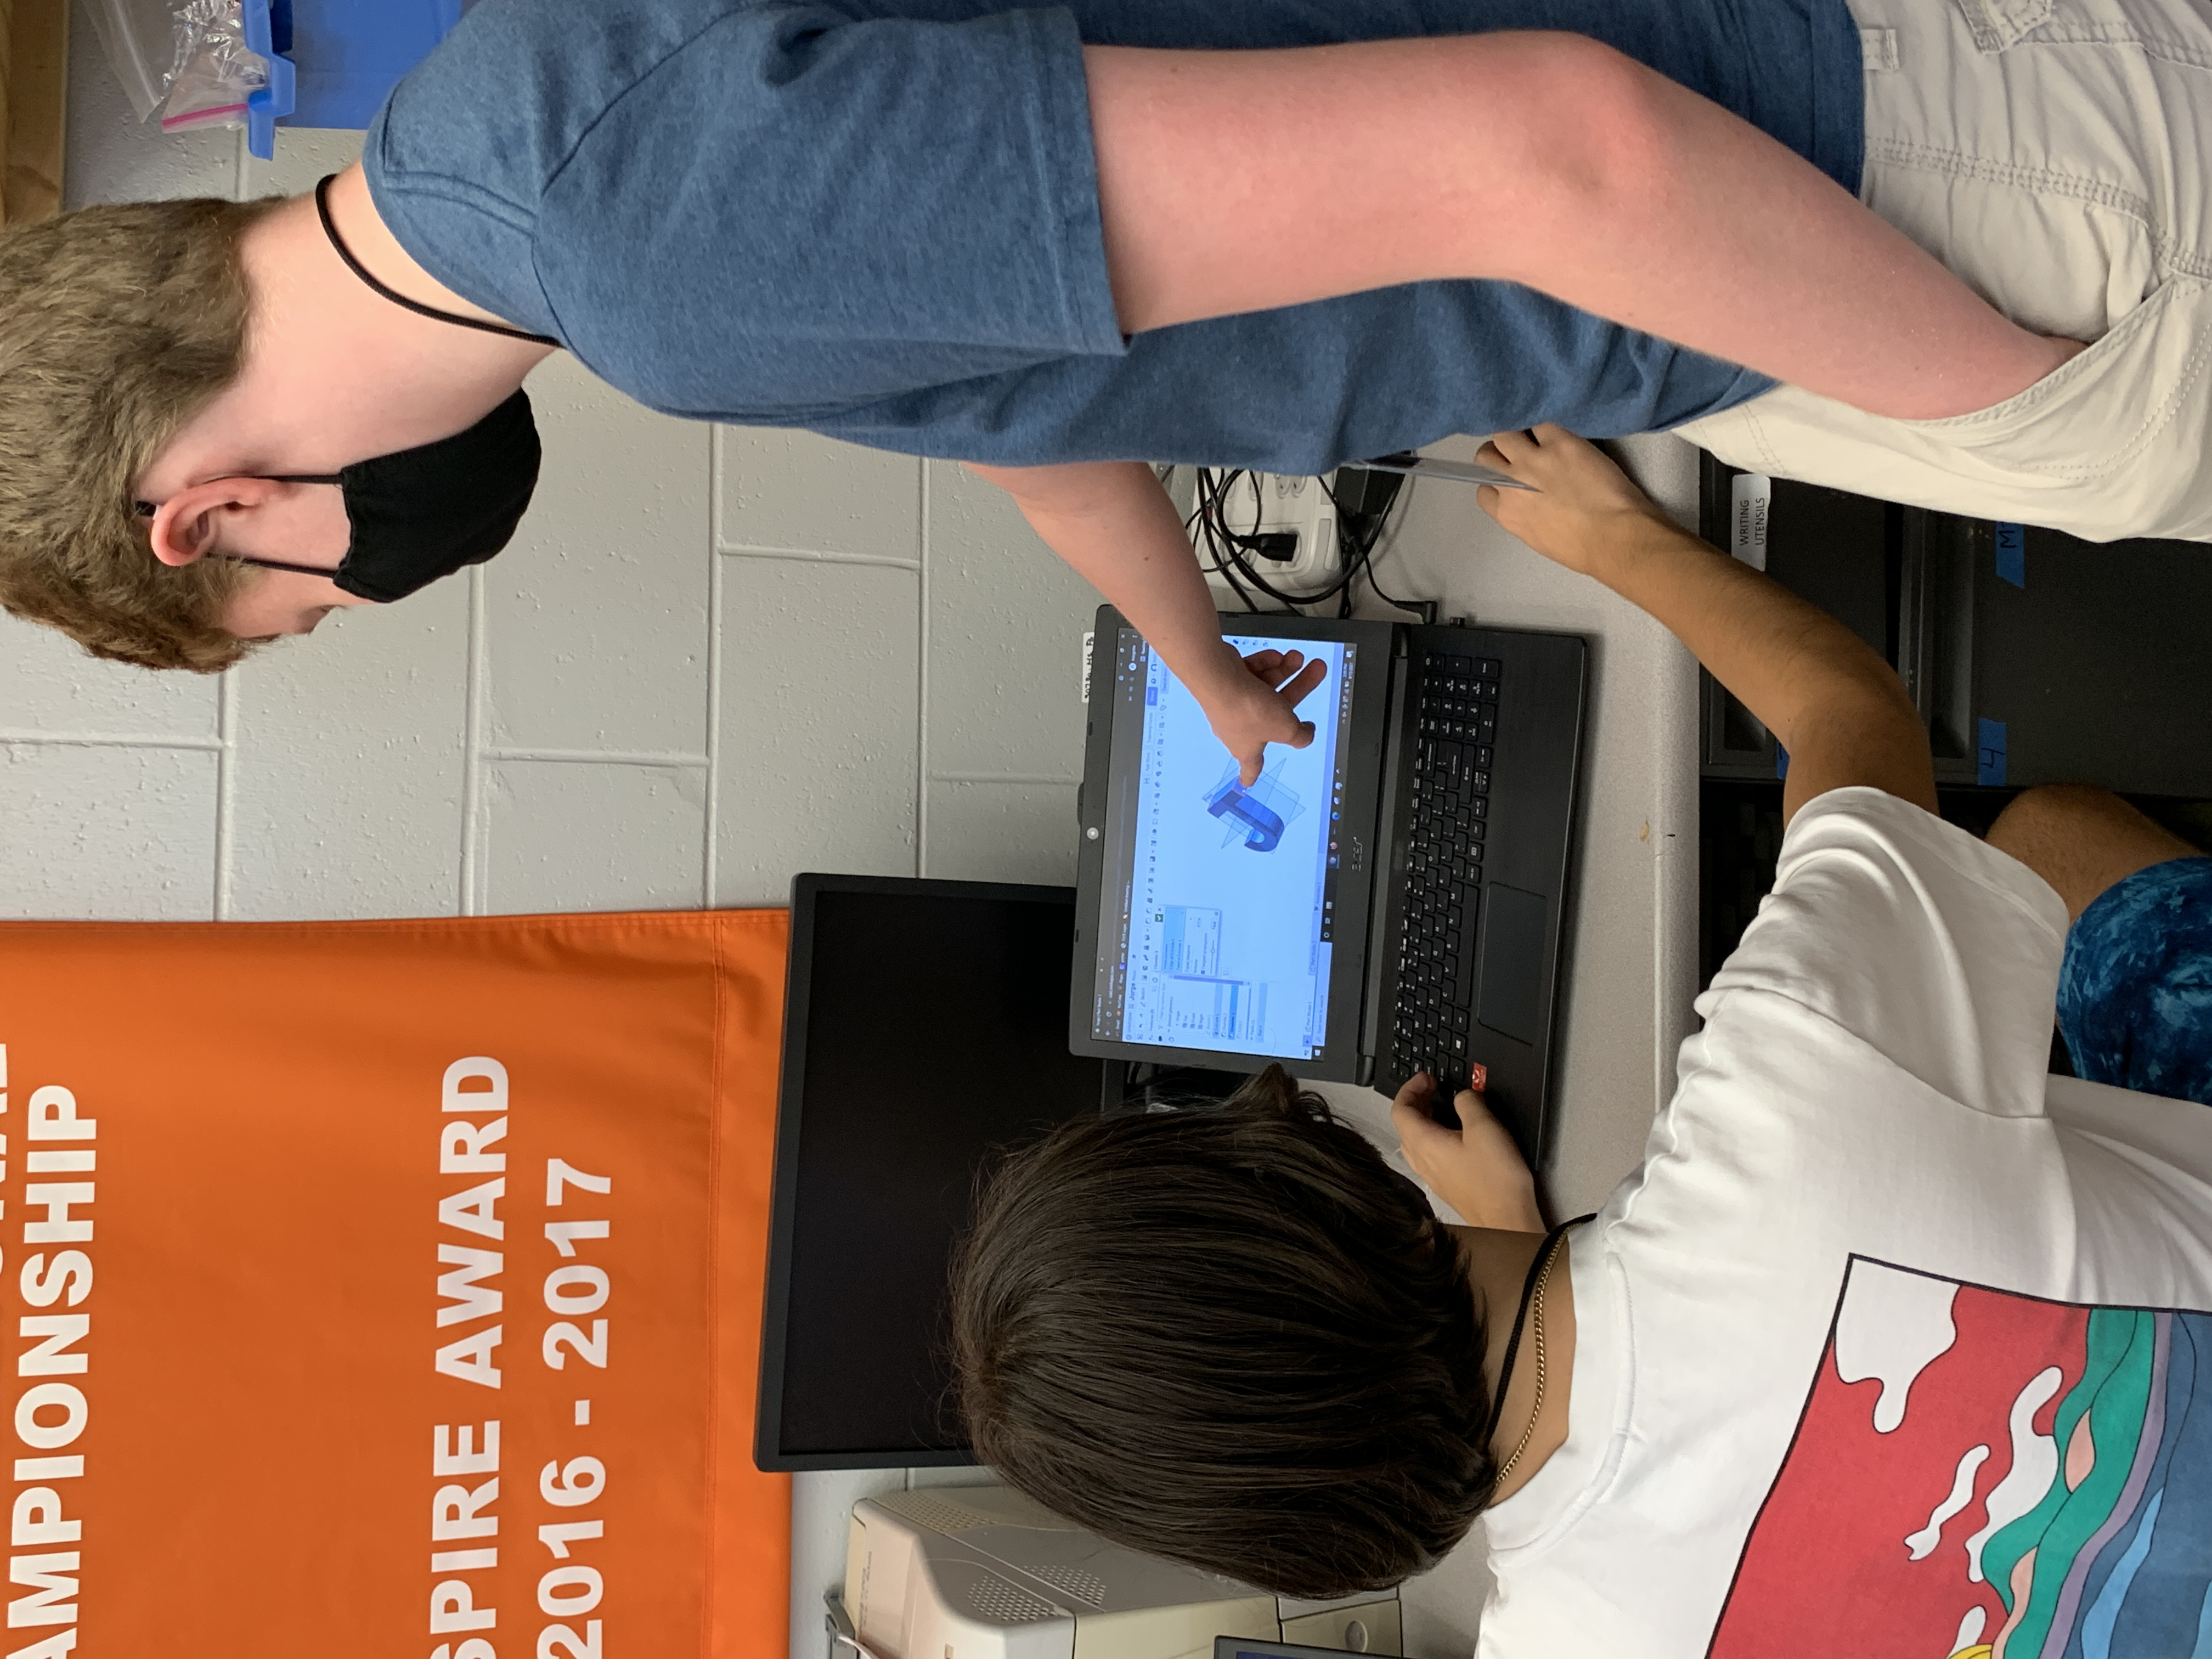
\includegraphics[width=0.8\textwidth]{Meetings/September/09-01-21/9-1-21_Program_Image2 - Nathan Forrer.JPG}
  \caption{Nathan helping Jorge}
  \label{fig:pic2}
\end{minipage}
\end{figure}

\begin{figure}[ht]
\centering
\begin{minipage}[b]{.50\textwidth}
  \centering
  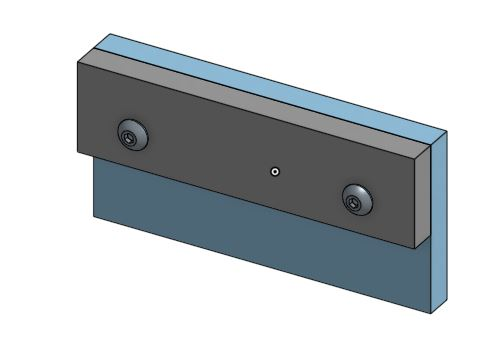
\includegraphics[width=0.8\textwidth]{Meetings/September/09-01-21/9-1-21_Program_Image3 - Nathan Forrer.JPG}
  \caption{CAD Picture}
  \label{fig:pic3}
\end{minipage}%
